\documentclass{article}
\usepackage[a4paper, top=3cm, bottom=2.5cm, left=2.5cm, right=2.5cm]{geometry}
\usepackage[spanish]{babel}
\usepackage[utf8]{inputenc}
\usepackage{tikz}
\usetikzlibrary{positioning, shapes.geometric}
\usepackage{titling}
\usepackage{graphicx}
\usepackage{fancyhdr}
\usepackage{amsmath}
\usepackage{amssymb}
\usepackage{multicol}
\usepackage{cancel}
\usepackage{setspace}
\usepackage{pgfplots}
\usepackage{hyperref}
\usepackage{float}
\pgfplotsset{compat=1.18}
\setlength{\parskip}{1em}
\setlength{\parindent}{0pt}


\pagestyle{fancy}
\fancyhf{}
\fancyhead[L]{
\includegraphics[width=2cm]{assets/logo-utp.png}}
\fancyhead[R]{\textbf{Introducción a las TIC}}

\fancyfoot[R]{\thepage}

\setlength{\textheight}{23cm}

\setlength{\headheight}{17.26935pt}
\addtolength{\topmargin}{-5.26935pt}
\setlength{\textheight}{23cm}


\title{
  
\includegraphics[width=5cm]{./assets/logo-utp.png} \\
  \vspace{1cm}
  \textbf{Universidad Tecnológica del Perú} \\
  \vspace{2cm}
  \textbf{Implementación de Soluciones TIC para la Optimización Operativa en la Bodega Morocco} \\
  \vspace{1cm}
  \large \textbf{Para el curso de Introducción a las Tecnologías de la Información y Comunicación} \\
}
\author{
  \begin{tabular}{ll}
    \textbf{Luis Huatay Salcedo.} & \texttt{hsluis4326@gmail.com} \\
    \textbf{Carlos Huari.} & \texttt{carlosplop123@gmail.com} \\
    \textbf{Jhocelin Jimenez.} & \texttt{nicollj49@gmail.com} \\
    \textbf{Eva Larico.} & \texttt{evalarico073@gmail.com} \\
    % \textbf{Kelvin Lázaro.} & \texttt{kelvinelb@gmail.com} \\
  \end{tabular} \\\\
  \texttt{Sección 24240}
}


% ENVIROMENTS

\begin{document}
\newgeometry{top=4cm}
\maketitle
\begin{center}
Docente Mg. Anita Condo Lopez.
\end{center}
\restoregeometry

\newpage 

\tableofcontents


\newpage

\section{Resumen}

  % En el presente informe se propone la implementación de soluciones TIC para optimizar la operativa de la Bodega Morocco, un negocio familiar dedicado a la venta de productos de primera necesidad en San Juan de Miraflores. La bodega enfrenta desafíos relacionados con la gestión manual de sus ventas y la falta de un control de inventario adecuado, lo que limita su capacidad para tomar decisiones informadas sobre las compras y la reposición de productos.

  % El objetivo general de la propuesta es automatizar el registro de ventas y la gestión de inventario de la bodega para reducir el tiempo empleado.  La solución propuesta incluye la implementación de un sistema de bases de datos para almacenar información sobre los productos, las ventas y el inventario de la bodega, el desarrollo de una interfaz de usuario intuitiva y fácil de usar para registrar las ventas y actualizar el inventario de forma automatizada, la generación de reportes periódicos sobre las ventas, el inventario y los productos más vendidos, la capacitación del personal de la bodega en el uso del nuevo sistema y la evaluación del impacto de la implementación de la solución TIC en la eficiencia operativa de la bodega y en la satisfacción del cliente.

  \begin{multicols}{2}
    \textbf{Resumen:} Este informe propone implementar soluciones TIC para mejorar la operación de la Bodega Morocco, un negocio familiar en San Juan de Miraflores. Actualmente, enfrenta problemas en la gestión manual de ventas y el control de inventario, lo que dificulta la toma de decisiones informadas.

    El objetivo principal es automatizar el registro de ventas e inventarios. La solución incluye un sistema de bases de datos para almacenar información, una interfaz de usuario sencilla para registrar ventas y actualizar inventarios, la generación de reportes periódicos y la capacitación del personal en el uso del sistema.

    \columnbreak

    \textbf{Abstract:} This report proposes implementing ICT solutions to optimize the operation of Bodega Morocco, a family business in San Juan de Miraflores. The bodega faces challenges in manual sales management and inadequate inventory control, limiting its ability to make informed decisions.

    The main objective is to automate sales and inventory management. The solution includes a database system to store data, an intuitive user interface for sales and inventory updates, periodic reports, and staff training on the new system.

\end{multicols}

\section{Marco Teórico}

  \subsection{Definición de TIC}

    Las Tecnologías de la Información y Comunicación (TIC) son un conjunto de herramientas, recursos y sistemas que permiten la adquisición, almacenamiento, procesamiento, transmisión y presentación de información de manera digital. Estas tecnologías han revolucionado la forma en que las personas se comunican, acceden a la información y realizan sus actividades diarias, transformando la sociedad y la economía en un entorno cada vez más digitalizado.

    Según Huidobro J. (2007) Se entiende un termino dilatado empleado para designar lo relativo a la informática conectada a Internet, y especialmente el aspecto social de éstos. Ya que Las nuevas tecnologías de la información y comunicación designan a la vez un conjunto de innovaciones tecnológicas pero también las herramientas que permiten una redefinición radical del funcionamiento de la sociedad.

    \begin{flushright}
      \textit{Huidobro J. (2007). Tecnologías de la información y la comunicación.}
    \end{flushright}



  \subsection{Importancia de las TIC}

    Las Tecnologías de la Información y Comunicación (TIC) juegan un papel fundamental en la sociedad actual, ya que han transformado la forma en que las personas se comunican, trabajan, estudian, se divierten y realizan sus actividades diarias. Algunas de las razones por las que las TIC son importantes son las siguientes:

    \begin{itemize}
      \item \textbf{Facilitan la comunicación:} Las TIC permiten a las personas comunicarse de forma rápida, eficiente y económica a través de diversos medios, como el correo electrónico, las redes sociales, las llamadas telefónicas, los mensajes de texto, entre otros. Esto ha acortado las distancias y ha facilitado la interacción entre individuos, empresas, organizaciones y gobiernos en todo el mundo.

      \item \textbf{Mejoran el acceso a la información:} Las TIC han democratizado el acceso a la información al permitir a las personas buscar, compartir y acceder a una amplia variedad de contenidos en línea. Esto ha contribuido a la educación, la investigación, el entretenimiento, etc.
      
      \item \textbf{Facilitan el trabajo colaborativo:} Las TIC permiten a las personas trabajar de forma colaborativa en tiempo real, independientemente de su ubicación geográfica. Herramientas como el correo electrónico, los sistemas de gestión de proyectos, las videoconferencias y las plataformas de colaboración en línea facilitan la comunicación y la coordinación entre equipos de trabajo.
      
      \item \textbf{Optimizan los procesos empresariales:} Las TIC han revolucionado la forma en que las empresas operan al permitir la automatización de procesos, la gestión eficiente de la información, la toma de decisiones basada en datos y la mejora de la productividad. Esto ha llevado a la creación de nuevos modelos de negocio, la optimización de tareas y la generación de nuevas oportunidades en el mercado.
      
      \item \textbf{Fomentan la innovación:} Las TIC son un motor de innovación en la sociedad al permitir el desarrollo de nuevas tecnologías, aplicaciones y servicios que mejoran la calidad de vida de las personas, impulsan el crecimiento económico y promueven el desarrollo sostenible. La tecnología ha transformado sectores como la salud, la educación, el transporte, la energía, la agricultura, entre otros, generando impactos positivos en la sociedad.
    \end{itemize}

\newpage 

\subsection{Antecedentes}

\begin{enumerate}
  \item \textbf{\textit{Implementación del sistema de ventas e inventario en Comercial Juanita, Aguas Verdes - Tumbes; 2021}}

  De acuerdo a Silva P. (2022). Comercial Juanita, es una empresa dedicada a la venta de productos agropecuarios, que se ha visto enfrentando a diversos desafíos al trabajar con un ineficiente sistema manual de ventas e inventario. El informe presente describirá todos los problemas encontrados en el negocio utilizando el sistema tradicional, tanto así, como las soluciones tecnológicas (TIC) que se implementaron para optimizar la eficiencia operativa. 
  
  \begin{itemize}
    \item \textbf{Problemas identificados:} 
    \begin{enumerate}
      \item \textbf{Registro manual de ventas:} Comercial Juanita, manejaba las ventas y el inventario mediante registros en cuadernos. Este método manual presentaba un gran riesgo ya que toda la información era almacenada en una libreta de apuntes, ocasionando así, confusiones y disgustos al cliente. Además, el rápido deterioro de los cuadernos presentaba un gran riesgo por la pérdida de datos. 
      \item \textbf{Confusiones y Errores en el inventario del negocio:} El sistema manual generaba muchos errores ya que no contaba con un control estructurado de los productos en su inventario. Esta falta de control de su inventario generaba confusión entre los empleados y muchas demoras en el proceso de venta, afectando a la satisfacción del cliente.   
      \item \textbf{Falta de un sistema de control:} Al depender netamente de registros físicos, no contaba con un mecanismo seguro para controlar el sistema de inventario o al menos garantizar la exactitud de la información. Este problema limitaba el seguimiento de ventas y el inventario, haciendo más frecuente la aparición de errores que afectaran sus operaciones diarias o su relación con su clientela. 
    \end{enumerate}
    \item \textbf{Herrmientas TIC implementadas:}
    \begin{enumerate}
      \item \textbf{Automatización de los procesos de venta:} Al implementar las TIC permitió la automatización de los registros de ventas y mejorar la gestión del inventario, eliminando la necesidad de registros manuales. Con un nuevo sistema, los datos se almacenan de manera digital, mejorando asi la eficiencia y la consulta de información 
      \item \textbf{Mejora en la eficiencia y rapidez:} Al implementar las TIC, redujo significativamente el tiempo de atención al cliente, debido al rápido acceso a los datos del inventario y también a que los empleados puedan visualizar en tiempo real a la disponibilidad de los productos. 
      \item \textbf{Sistema Centralizado de Inventario Seguro:} El nuevo sistema cuenta con una base de datos que centraliza toda la información de ventas e inventario. Este cambio facilita el almacenamiento del historial de sus clientes y todas sus compras, tambien permite un control efectivo de los productos disponibles. La empresa ahora puede rastrear las transacciones de forma segura, minimizando los errores y reforzando la seguridad de su información.  
      \item \textbf{Metodología utilizada:} Comercial Juanita utilizo la metodología RUP (Rational Unifed Process) y UML (Lenguaje unificado de modelado). Estas metodologías estructuran y organizan todos los procesos del sistema, permitiendo un diseño adecuado de la base de datos y de interfaces de usuario. 
    \end{enumerate} 
  \end{itemize}
  \newpage
  \item \textbf{\textit{Implementación de un sistema para el control de inventario y ventas de la tienda Comercial de Ropa Novedades Yohanny - Talara; 2018}}
  
  Por Ramirez R. (2018) El informe presenta una tesis de ingeniería de sistemas que propone la implementación de un sistema de control de inventario y ventas para la tienda de ropa "Novedades Yohanny" en Talara, Perú. La investigación, de tipo cuantitativa y descriptiva, analiza la satisfacción de empleados y clientes con los procesos actuales y la aceptación de la nueva propuesta. Los resultados muestran una alta necesidad de mejora en los procesos existentes y una gran aceptación del sistema propuesto. La tesis detalla el diseño del sistema, incluyendo modelos UML y la tecnología a utilizar (PHP y MySQL).

\begin{itemize}
  \item \textbf{Problemas identificados:} 
  \begin{enumerate}
    \item \textbf{Problemas en el almacén:} Conteo manual de la mercadería: Cuando llega nueva mercadería, se realiza un conteo manual para establecer el stock disponible para la venta. Sin embargo, la mercadería se va sacando del almacén sin contabilizar la cantidad, lo que ocasiona que cada seis meses se tenga que realizar un nuevo conteo, lo que genera pérdida de tiempo.
    \item \textbf{Mala distribución de la mercadería:} Existe desorden en la ubicación de la ropa en el almacén, lo que causa confusión y pérdida de tiempo al buscar la mercadería. Esto también genera problemas cuando un cliente solicita un producto que no se encuentra en la tienda, ya que se pierde tiempo buscándolo en el almacén.
    \item \textbf{Procesos manuales:} Las boletas y consultas se realizan de forma manual, así como los cálculos, lo que puede ocasionar errores que resultan en descuentos para los trabajadores. Conteo manual del monto vendido: Al final del día, se realiza un conteo manual del monto vendido para compararlo con las boletas, lo que consume mucho tiempo y puede generar discrepancias.
    \item \textbf{Conteo manual del monto vendido:} Al final del día, se realiza un conteo manual del monto vendido para compararlo con las boletas, lo que consume mucho tiempo y puede generar discrepancias.
  \end{enumerate}
  \item \textbf{Herrmientas TIC implementadas:}
  \begin{enumerate}
    \item \textbf{RUP (Rational Unified Process):} Este método de desarrollo se caracteriza por ser iterativo e incremental, centrado en la arquitectura del sistema y en la aplicación de buenas prácticas de ingeniería de software.
    \item \textbf{UML (Unified Modeling Language):} Este lenguaje de modelado estándar se utiliza para visualizar, especificar, construir y documentar los diferentes componentes del sistema. Se basa en la creación de diagramas para representar los diferentes aspectos del software, como los casos de uso, las clases, las actividades y las interacciones entre los objetos.
    \item \textbf{PHP:} Un lenguaje de programación de código abierto especialmente adecuado para el desarrollo web. Se utiliza para crear páginas web dinámicas que interactúan con bases de datos.
    \item \textbf{MySQL:} Un sistema de gestión de bases de datos relacional de código abierto. Es conocido por su rapidez, solidez y flexibilidad. Se utiliza ampliamente en aplicaciones web y se integra fácilmente con PHP.
    \item \textbf{Servidor web:} No se especifica en las fuentes si se utilizará un servidor web en particular. Sin embargo, dado que se empleará PHP como lenguaje de programación, es probable que se utilice un servidor web compatible con este lenguaje, como Apache.
  \end{enumerate}
\end{itemize}


\end{enumerate}

\newpage
\section{Descripción de la Empresa}

  \begin{spacing}{1.5}
    \noindent
    \textbf{Nombre de la Empresa:} Bodega Morocco \\
    \textbf{Giro de la Empresa:} Venta de productos de primera necesidad \\
    \textbf{Correo Electrónico:} bodegaMorocco@gmail.com \\
    \textbf{Teléfono:} 987654321
  \end{spacing}

  La Bodega Morocco es un negocio familiar que ha servido a la comunidad de San Juan de Miraflores, específicamente en el sector 12 de noviembre de Pamplona Alta, por más de una década. A pesar de su tamaño modesto, la bodega ha logrado ganarse la confianza de los vecinos por su atención cercana y productos de calidad. El establecimiento ofrece una variedad de productos básicos que cubren las necesidades diarias de sus clientes, tales como arroz, azúcar, bebidas, enlatados y productos de limpieza. Estos productos son esenciales para los hogares de la zona, y la atención al cliente es únicamente presencial, lo que refuerza la relación directa con su clientela.

  Actualmente, la Bodega Morocco opera desde un único local. A pesar de las limitaciones en infraestructura, los dueños buscan constantemente mejorar sus servicios para agilizar los procesos de compra y brindar una mejor experiencia a sus clientes. La bodega ha experimentado un crecimiento constante en los últimos años, lo que ha llevado a los dueños a considerar la posibilidad de expandir su negocio. Sin embargo, antes de tomar esta decisión, desean optimizar sus operaciones actuales para garantizar que puedan manejar un mayor volumen de ventas sin comprometer la calidad de su servicio.

  Así mismo, en relación con el aumento del volumen de venta y la necesidad de mejorar la atención al cliente, los propietarios de la bodega han identificado la necesidad de implementar soluciones tecnológicas que les permitan automatizar los procesos de venta y mejorar el control de inventario. La gestión manual de las ventas y el inventario ha demostrado ser ineficiente y propensa a errores, lo que ha llevado a la acumulación de productos no vendidos y a la falta de stock de artículos esenciales. La implementación de un sistema digital permitirá a los dueños de la bodega llevar un control más preciso y eficiente de sus ventas diarias, así como obtener una visión clara del estado del inventario. Esto facilitará la toma de decisiones informadas en cuanto a la reposición de productos, evitando tanto la falta de stock como la acumulación innecesaria de mercancías.

\newpage
\section{Problemática}

  La bodega Morocco enfrenta un desafío relacionado con la gestión manual de sus ventas y la falta de un control de inventario adecuado. Los constantes errores en los registros manuales de las transacciones diarias, la falta de un sistema automatizado de inventario y la ausencia de un sistema digital para analizar patrones de consumo han llevado a la acumulación de productos no vendidos y a la falta de stock de artículos esenciales. Esto afecta tanto la calidad del servicio como la satisfacción del cliente, lo que a su vez limita el crecimiento y la expansión del negocio.

  Es importante entender que esta como otras bodegas, son negocios que se encuentran en constante competencia con otros establecimientos similares, por lo que la eficiencia operativa y la calidad del servicio son factores clave para mantenerse competitivos en el mercado. La implementación de soluciones tecnológicas, como un sistema de registro de ventas y un sistema de control de inventario, permitirá a la bodega mejorar su eficiencia operativa, reducir los errores

  \subsection{Procesos Manuales de venta e inventario:}

  Actualmente, la Bodega Morocco presenta dificultades con la gestión manual de sus ventas y la falta de un control de inventario adecuado. Los propietarios llevan un registro manual de las transacciones diarias, lo que implica un proceso laborioso, propenso a errores y que consume un tiempo considerable. Esta metodología limita su capacidad para tomar decisiones rápidas y eficaces sobre las compras y la reposición de productos.

  La ausencia de un sistema automatizado de inventario complica aún más la identificación de los artículos que se están agotando o aquellos con alta demanda. Esto puede reProcesos Manuales de venta e inventario:sultar en una pérdida de oportunidades de venta y en la insatisfacción de los clientes al no encontrar productos disponibles. Además, la falta de un sistema digital impide analizar patrones de consumo, lo que dificulta la planificación de compras futuras. Sin una visión clara de los productos con mayor o menor rotación, es más probable que se acumulen productos no vendidos o se agoten artículos esenciales, afectando tanto la calidad del servicio como la satisfacción del cliente.

  \subsection{Problemas con el stock derivado de la falta de control de inventario:}

  La falta de un control de inventario adecuado ha llevado a la acumulación de productos no vendidos y a la falta de stock de artículos esenciales. Los propietarios de la bodega no tienen una visión clara del estado del inventario, lo que dificulta la toma de decisiones informadas sobre la reposición de productos. Esto puede resultar en la acumulación innecesaria de mercancías, lo que afecta la rentabilidad del negocio, o en la falta de stock de productos esenciales, lo que afecta la satisfacción del cliente.

  La gestión manual del inventario también ha demostrado ser propensa a errores, lo que puede llevar a discrepancias en los registros y a la pérdida de productos. La falta de un sistema automatizado de inventario dificulta la identificación de los productos con mayor o menor rotación, lo que limita la capacidad de los propietarios para planificar las compras de reposición de forma eficiente. Esto puede resultar en la falta de stock de artículos esenciales en momentos críticos, lo que afecta la calidad del servicio y la satisfacción del cliente.

\newpage

\section{Desarrollo de la situación planteada}
    
    Hacer uso de las distintas herramientas TIC estudiadas durante el presente ciclo académico para la implementación de un sistema de control de inventario y ventas en la Bodega Morocco, con el fin de optimizar la operativa del negocio y mejorar la satisfacción del cliente.

  \textbf{Objetivos:}
    \begin{itemize}
      \item \textbf{Implementar} un sistema de bases de datos relacional del tipo MySQL para almacenar información sobre los productos, las ventas y el inventario de la bodega. Esto a fin de facilitar el acceso a los datos y la generación de informes detallados sobre el desempeño del negocio. Consideramos que esta RBDMS es la más adecuada para el almacenamiento de datos en la bodega, ya que es un sistema robusto, escalable y de código abierto que permite gestionar grandes volúmenes de información de forma eficiente.
        
      \item \textbf{Desarrollar} una interfaz de usuario intuitiva y fácil de usar para registrar las ventas y actualizar el inventario de forma automatizada. Esta interfaz que se vale de los gráficos generados digitalmente permitirá a los empleados de la bodega ingresar los datos de los productos vendidos, calcular el monto total de la venta y actualizar el inventario de forma automática. La interfaz estará diseñada de forma sencilla y amigable, con botones y campos de texto claros y fáciles de entender. Además, se implementarán validaciones para garantizar la integridad de los datos ingresados y se incluirán mensajes de error en caso de que se produzcan errores en la entrada de datos.
        
      \item \textbf{Generar} reportes periódicos sobre las ventas, el inventario y los productos más vendidos para facilitar la toma de decisiones. Estos reportes producto de una buena gestión de las texnologías de la información proporcionarán una visión clara del desempeño del negocio y permitirán identificar oportunidades de mejora. Los reportes se generarán de forma automática a partir de los datos almacenados en la base de datos y se presentarán de forma estructurada y visual para facilitar su interpretación. Los propietarios de la bodega podrán acceder a los reportes a través de la interfaz de usuario y consultar la información de forma rápida y precisa.
        
      \item \textbf{Capacitar} al personal de la bodega en el uso del nuevo sistema y brindar soporte técnico continuo para garantizar su correcto funcionamiento. La capacitación se realizará de forma presencial y práctica, con ejemplos y ejercicios que permitan a los empleados familiarizarse con la interfaz de usuario y las funcionalidades del sistema. Además, se establecerá un canal de comunición como pueden ser por correo, redes sociales, etc, para que los empleados puedan reportar cualquier problema o duda que surja durante el uso del sistema y recibir asistencia técnica oportuna.
        
      \item \textbf{Evaluar} el impacto de la implementación de la solución TIC en la eficiencia operativa de la bodega y en la satisfacción del cliente. Se realizarán encuestas de satisfacción a los clientes para recopilar sus opiniones sobre el nuevo sistema y se analizarán los datos obtenidos de tal manera que podamos entender como estos surgen en un ecosistema de BD relacional, esto a fin de medir el desempeño del negocio en la solución TIC. Los propietarios de la bodega utilizarán esta información para identificar áreas de mejora y realizar ajustes en el sistema en caso de ser necesario.
    \end{itemize}
    

\newpage

\section{Herramientas TIC a Emplear}

  Para la implementación de la solución propuesta, se utilizarán las siguientes herramientas TIC:

  \subsection{Sistema de Gestión de Bases de Datos (SGBD)}

    Un Sistema de Gestión de Bases de Datos (SGBD) es un software que permite almacenar, gestionar y recuperar información de una base de datos de forma eficiente y segura. En este caso, se utilizará MySQL como SGBD para almacenar información sobre los productos, las ventas y el inventario de la bodega. MySQL es un sistema de gestión de bases de datos relacional de código abierto que ofrece un alto rendimiento, escalabilidad y fiabilidad. Permite gestionar grandes volúmenes de datos de forma eficiente y proporciona una amplia gama de funcionalidades para el almacenamiento, la consulta y la administración de la información.

\vspace{-0.5cm}
  \subsection{Tenologías WEB}

    Una Aplicación Web es un programa informático que se ejecuta en un navegador web y que permite a los usuarios interactuar con una base de datos a través de una interfaz gráfica. En este caso, se desarrollará una aplicación web para que los empleados de la bodega puedan registrar las ventas de forma automatizada. La aplicación permitirá ingresar los datos de los productos vendidos, calcular el monto total de la venta y actualizar el inventario de forma automática.

  \subsection{Lenguajes de Programación}

    Para el desarrollo de la aplicación web, se utilizarán los siguientes lenguajes de programación:

    \begin{itemize}
      \item \textbf{HTML:} Lenguaje de marcado que se utiliza para crear la estructura y el contenido de las páginas web.
      \item \textbf{CSS:} Lenguaje de estilos que se utiliza para dar formato y diseño a las páginas web.
      \item \textbf{JavaScript:} Lenguaje de programación que se utiliza para añadir interactividad y dinamismo a las páginas web.
      \item \textbf{PHP:} Lenguaje de programación de código abierto que se utiliza para crear aplicaciones web dinámicas y conectarse a bases de datos.
    \end{itemize}

    Estos lenguajes de programación se utilizarán para desarrollar la interfaz de usuario de la aplicación web y para conectarla con la base de datos de MySQL. Se utilizarán las tecnologías web para crear una interfaz de usuario intuitiva y fácil de usar que permita a los empleados de la bodega registrar las ventas y actualizar el inventario de forma automatizada.
\vspace{-0.5cm}
  \subsection{Herramientas de Diseño}

    Para el diseño de la interfaz de usuario de la aplicación web, se utilizarán las siguientes herramientas:

    \begin{itemize}
      \item \textbf{Bizagi:} Herramienta de modelado de procesos de negocio que se utiliza para diseñar, documentar y optimizar los procesos de negocio de forma visual y colaborativa.
      \item \textbf{Figma:} Herramienta de diseño de interfaces de usuario que se utiliza para crear diseños de alta fidelidad y colaborar en tiempo real con otros diseñadores.
    \end{itemize}

\newpage

\section{Plan de implementación de la solución}

% 1. Análisis y Planificación (2 semanas)
% 	•	Reunión con los dueños para identificar requerimientos específicos.
% 	•	Estudio detallado de los procesos actuales (manuales).
% 	•	Selección de las herramientas TIC (bases de datos, aplicación web, etc.).

% 2. Diseño del Sistema (3 semanas)
% 	•	Creación de prototipos para la aplicación web y el sistema de inventario.
% 	•	Diseño de la base de datos para registrar ventas, inventario y reportes.
% 	•	Validación del diseño con los dueños de la bodega.

% 3. Desarrollo e Integración (4 semanas)
% 	•	Programación de la aplicación web (interfaz y backend).
% 	•	Implementación de la base de datos (SGBD).
% 	•	Integración del sistema de inventario y generación de reportes.

% 4. Pruebas (2 semanas)
% 	•	Verificación funcional de la aplicación web y el sistema de inventario.
% 	•	Simulación de procesos reales para detectar errores.
% 	•	Ajustes según los resultados de las pruebas.

% 5. Capacitación (1 semana)
% 	•	Formación del personal en el uso del sistema.
% 	•	Guías prácticas y soporte inicial.

% 6. Implementación y Seguimiento (2 semanas)
% 	•	Instalación del sistema en la bodega.
% 	•	Monitoreo del desempeño y solución de problemas iniciales.

% Diagrama de Gantt

% Se presenta el cronograma detallado con las actividades y tiempos estimados:

% Duración Total: 14 semanas

% Actividades	Semana 1	Semana 2	Semana 3	Semana 4	Semana 5	Semana 6	Semana 7	Semana 8	Semana 9	Semana 10	Semana 11	Semana 12	Semana 13	Semana 14
% Análisis y Planificación	X	X												
% Diseño del Sistema			X	X	X									
% Desarrollo e Integración					X	X	X	X						
% Pruebas									X	X				
% Capacitación											X			
% Implementación y Seguimiento												X	X

Se establecen los siguientes pasos para la implementación de la solución propuesta:

\subsection{Análisis y Planificación (2 semanas)}

  \begin{itemize}
    \item Reunión con los dueños para identificar requerimientos específicos.
    \item Estudio detallado de los procesos actuales (manuales).
    \item Selección de las herramientas TIC (bases de datos, aplicación web, etc.).
  \end{itemize}

\subsection{Diseño del Sistema (3 semanas)}
  
    \begin{itemize}
      \item Creación de prototipos para la aplicación web y el sistema de inventario.
      \item Diseño de la base de datos para registrar ventas, inventario y reportes.
      \item Validación del diseño con los dueños de la bodega.
    \end{itemize}

\subsection{Desarrollo e Integración (4 semanas)}

    \begin{itemize}
      \item Programación de la aplicación web (interfaz y backend).
      \item Implementación de la base de datos (SGBD).
      \item Integración del sistema de inventario y generación de reportes.
    \end{itemize}

\subsection{Pruebas (2 semanas)}

    \begin{itemize}
      \item Verificación funcional de la aplicación web y el sistema de inventario.
      \item Simulación de procesos reales para detectar errores.
      \item Ajustes según los resultados de las pruebas.
    \end{itemize}

\subsection{Capacitación (1 semana)}

    \begin{itemize}
      \item Formación del personal en el uso del sistema.
      \item Guías prácticas y soporte inicial.
    \end{itemize}


\subsection{Implementación y Seguimiento (2 semanas)}


    \begin{itemize}
      \item Instalación del sistema en la bodega.
      \item Monitoreo del desempeño y solución de problemas iniciales.
    \end{itemize}

\newpage

El diagrama de Gantt muestra el cronograma detallado con las actividades y tiempos estimados para la implementación de la solución propuesta. El proceso se llevará a cabo en un total de 14 semanas, dividiendo las tareas en seis etapas: Análisis y Planificación, Diseño del Sistema, Desarrollo e Integración, Pruebas, Capacitación, Implementación y Seguimiento.
\begin{figure}[H]
  \centering
  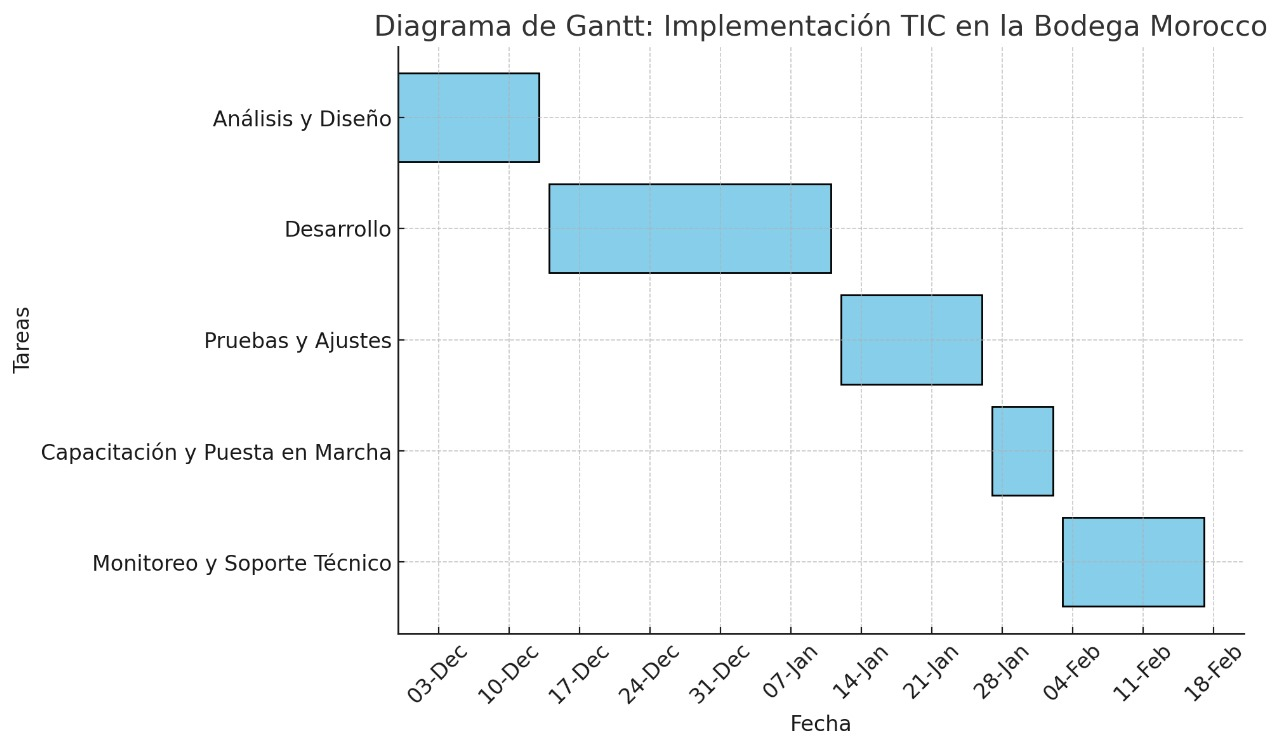
\includegraphics[width=0.8\textwidth]{./assets/gantt.jpeg}
  \caption{Diagrama de Gantt.}
\end{figure}

Proceso de login. Este algoritmo se encarga de verificar si el usuario y la contraseña ingresados son correctos. Si el usuario y la contraseña son correctos, se redirige al usuario a la página de inicio. Si el usuario y la contraseña son incorrectos, se muestra un mensaje de error y se le da la opción de intentarlo de nuevo.

\begin{figure}[H]
  \centering
  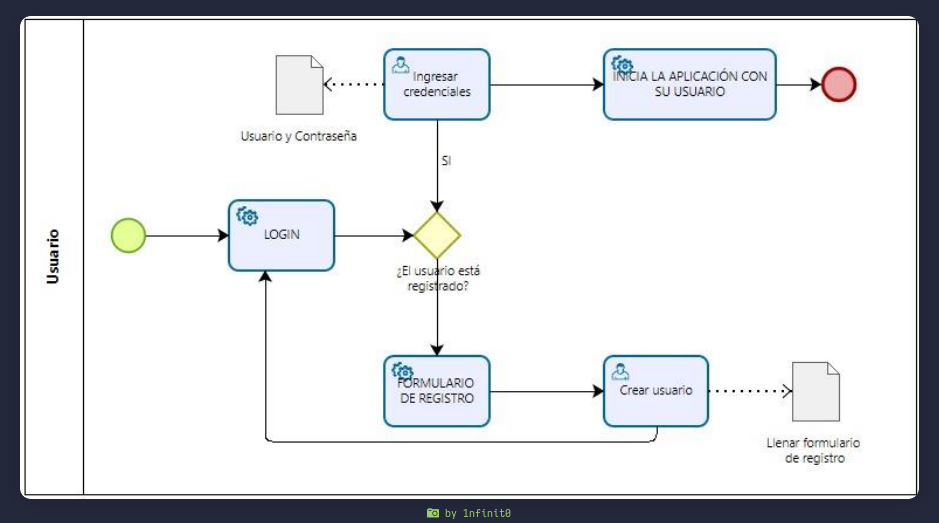
\includegraphics[width=0.8\textwidth]{./assets/p-login.png}
  \caption{Proceso de login.}
\end{figure}

\newpage

Proceso del registro de un cliente. Este algoritmo se encarga de registrar un nuevo cliente en la base de datos. El usuario ingresa los datos del cliente, como el nombre, la dirección y el número de teléfono, y se almacenan en la base de datos. Una vez que se ha registrado el cliente, se muestra un mensaje de confirmación y se redirige al usuario a la página de inicio.

\begin{figure}[H]
  \centering
  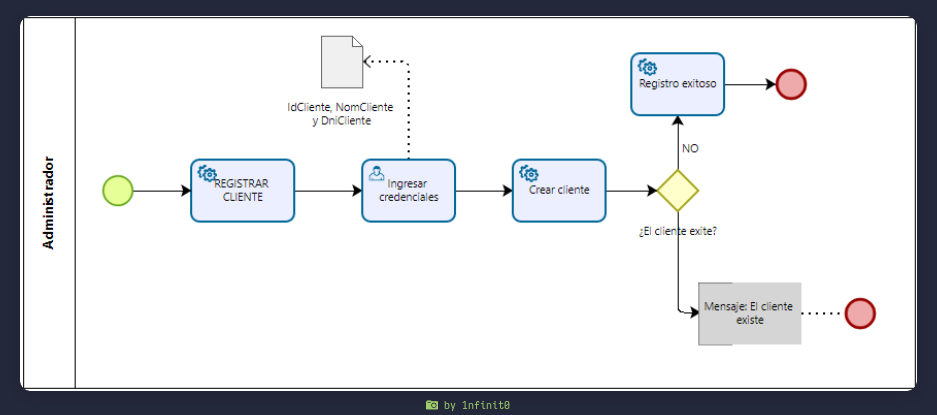
\includegraphics[width=0.8\textwidth]{./assets/p-clientes.png}
  \caption{Proceso del registro de un cliente.}
\end{figure}

\newpage

\textbf{\large{Diagrama entidad-relación de la base de datos:}}

\begin{center}
  \begin{tikzpicture}[
    entity/.style={draw, rectangle, rounded corners, fill=blue!20, text centered, minimum width=6cm, minimum height=1.5cm},
    attribute/.style={text width=5cm, align=left},
    relationship/.style={draw, diamond, fill=red!20, text centered, minimum width=2.5cm, minimum height=1.5cm},
    line/.style={-latex, thick},
    title/.style={font=\bfseries, yshift=0cm}, % Aumentar el desplazamiento
    node distance=1cm % Aumentar la distancia entre los nodos
  ]
  
  % Entidades
  \node[entity] (producto) {
      \begin{tabular}{ll}
          \textbf{Atributo} & \textbf{Tipo} \\
          ID Producto       & INT           \\
          Nombre            & VARCHAR(100)  \\
          Descripción       & TEXT          \\
          Precio            & DECIMAL(10,2) \\
      \end{tabular}
  };
  \node[above=of producto, title] {Producto};
  
  \node[entity, right=of producto] (venta) {
      \begin{tabular}{ll}
          \textbf{Atributo} & \textbf{Tipo} \\
          ID Venta          & INT           \\
          ID Producto       & INT (FK)      \\
          Fecha             & DATE          \\
          Cantidad          & INT           \\
          Total             & DECIMAL(10,2) \\
      \end{tabular}
  };
  \node[above=of venta, title] {Venta};
  
  \node[entity, below=of producto] (inventario) {
      \begin{tabular}{ll}
          \textbf{Atributo} & \textbf{Tipo} \\
          ID Inventario     & INT           \\
          ID Producto       & INT (FK)      \\
          Stock Inicial     & INT           \\
          Stock Actual      & INT           \\
          Umbral Reposición & INT           \\
      \end{tabular}
  };
  
  % Relaciones
  \draw[line] (producto) -- node[above] {1} (venta);
  \draw[line] (venta) -- node[below] {N} (producto);
  \draw[line] (producto) -- node[below] {1} (inventario);
  \draw[line] (inventario) -- node[above] {N} (producto);
  
  \end{tikzpicture}
\end{center}

\section{Prototipado de las soluciones}

A continuación se muestra un prototipo de login para el control del inventario de la Bodega Morocco. Esta aplicación web permitirá a los empleados de la bodega acceder al sistema de control de inventario y registrar las ventas de forma automatizada.

% imágenes:

\begin{figure}[H]
  \centering
  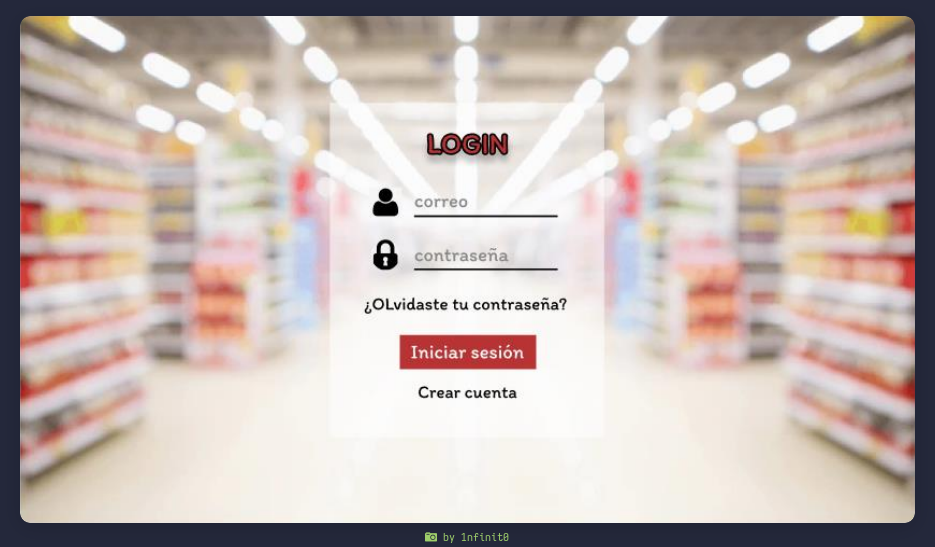
\includegraphics[width=0.7\textwidth]{./assets/login.png}
  \caption{Prototipo de login}
\end{figure}

Pantalla de inicio de sesión. En esta pantalla, los empleados de la bodega podrán ingresar su nombre de usuario y contraseña para acceder al sistema de control de inventario. Si los datos son correctos, se les redirigirá a la página de inicio. Si los datos son incorrectos, se mostrará un mensaje de error y se les dará la opción de intentarlo de nuevo.

\begin{figure}[H]
  \centering
  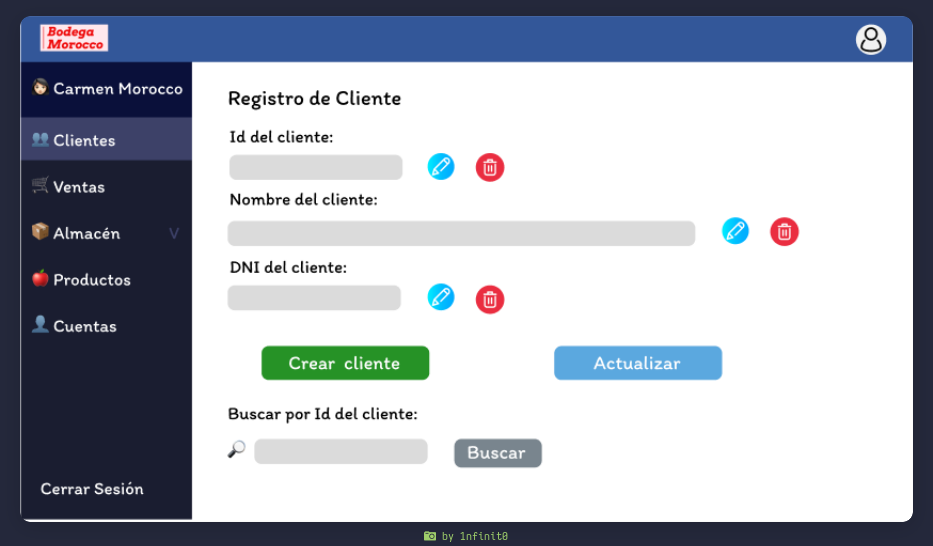
\includegraphics[width=0.8\textwidth]{./assets/registro.png}
  \caption{Prototipo del registro de clientes.}
\end{figure}

Vista de la página de registro de clientes. En esta página, los empleados de la bodega podrán ingresar los datos de los clientes, como el nombre, la dirección y el número de teléfono, y registrarlos en la base de datos. La interfaz estará diseñada de forma sencilla y amigable, con campos de texto claros y fáciles de entender.

\begin{figure}[H]
  \centering
  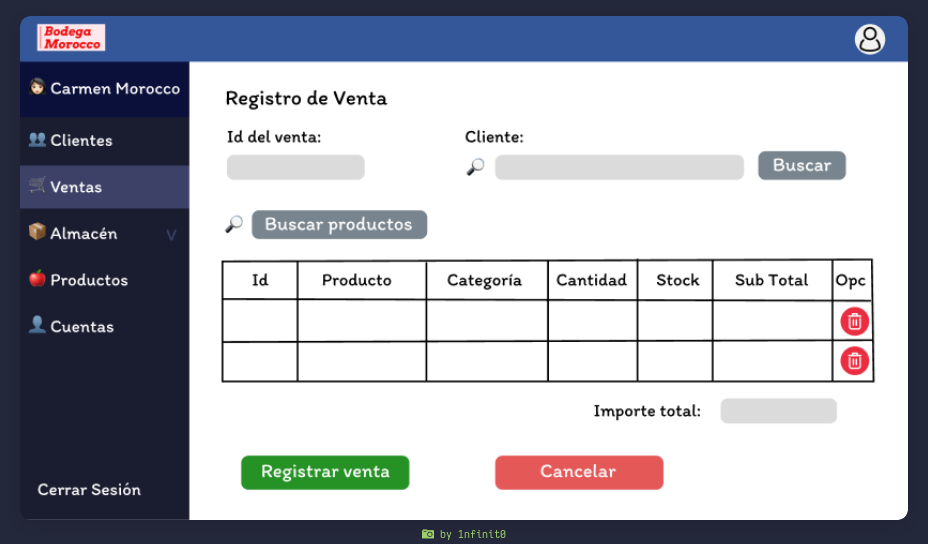
\includegraphics[width=0.8\textwidth]{./assets/venta.png}
  \caption{Prototipo del registro de ventas.}
\end{figure}

Vista de la página de registro de ventas. En esta página, los empleados de la bodega podrán ingresar los datos de los productos vendidos, calcular el monto total de la venta y actualizar el inventario de forma automática. La interfaz estará diseñada de forma sencilla y amigable, con botones y campos de texto claros y fáciles de entender.

\newpage

\section{Conclusiones}

La implementación de un sistema de control de inventario y ventas en la Bodega Morocco no solo optimizará la operativa del negocio, sino que también mejorará la satisfacción del cliente. La automatización de los procesos de venta y la gestión de inventarios contribuirá a reducir los errores y a mejorar la precisión de las operaciones diarias.

El uso de herramientas TIC como MySQL, PHP, HTML, CSS y JavaScript bajo un marco de trabajo establecido con VS Code, permitirá el desarrollo de una aplicación web intuitiva y fácil de usar, facilitando tanto el registro de ventas como la actualización automatizada del inventario. Además, la generación de reportes periódicos sobre ventas, inventarios y productos más vendidos proporcionará una visión clara del desempeño del negocio, lo que ayudará a identificar áreas de mejora y optimización.

La capacitación del personal en el uso del sistema, junto con el soporte técnico continuo, será crucial para garantizar el funcionamiento eficiente de la solución, así como su aceptación por parte de los empleados. Asimismo, la evaluación del impacto de la implementación, tanto en la eficiencia operativa como en la satisfacción del cliente, permitirá detectar posibles áreas de ajuste y realizar mejoras continuas.

En resumen, la implementación de un sistema de control de inventario y ventas en la Bodega Morocco representa una solución tecnológica que no solo mejorará la eficiencia operativa, sino también la experiencia del cliente. La integración de herramientas TIC adecuadas y la capacitación del personal son fundamentales para asegurar el éxito del proyecto y la aceptación del nuevo sistema.

  \begin{thebibliography}{}

    \bibitem{Huidobro} 
    Huidobro, J. (2007). \textit{Tecnologías de la información y la comunicación}. Universidad Politécnica de Madrid.
    
    \bibitem{Silva} 
    Silva, P. (2022). \textit{Implementación del sistema de ventas e inventario en Comercial Juanita, Aguas Verdes - Tumbes}. Universidad Nacional de Tumbes.
    
    \bibitem{Ramirez} 
    Ramírez, R. (2018). \textit{Implementación de un sistema para el control de inventario y ventas de la tienda Comercial de Ropa Novedades Yohanny - Talara}. Universidad Nacional de Talara.
    
    \end{thebibliography}
    
\end{document}